\append{Графічний інтерфейс користувача}
\label{appendix: A}

Розробка програмного забезпечення охоплювала як імплементацію ітераційних формул переоцінки параметрів моделі, так і розробку графічного інтерфейсу користувача для ефективного керування різними блоками коду. 

Наприклад, на малюнку нижче продемонстровано задання необхідних вхідних даних для генерування відповідного ланцюга Маркова для подальшого розв'язання задачі локалізації.

\begin{figure}[H]\centering
    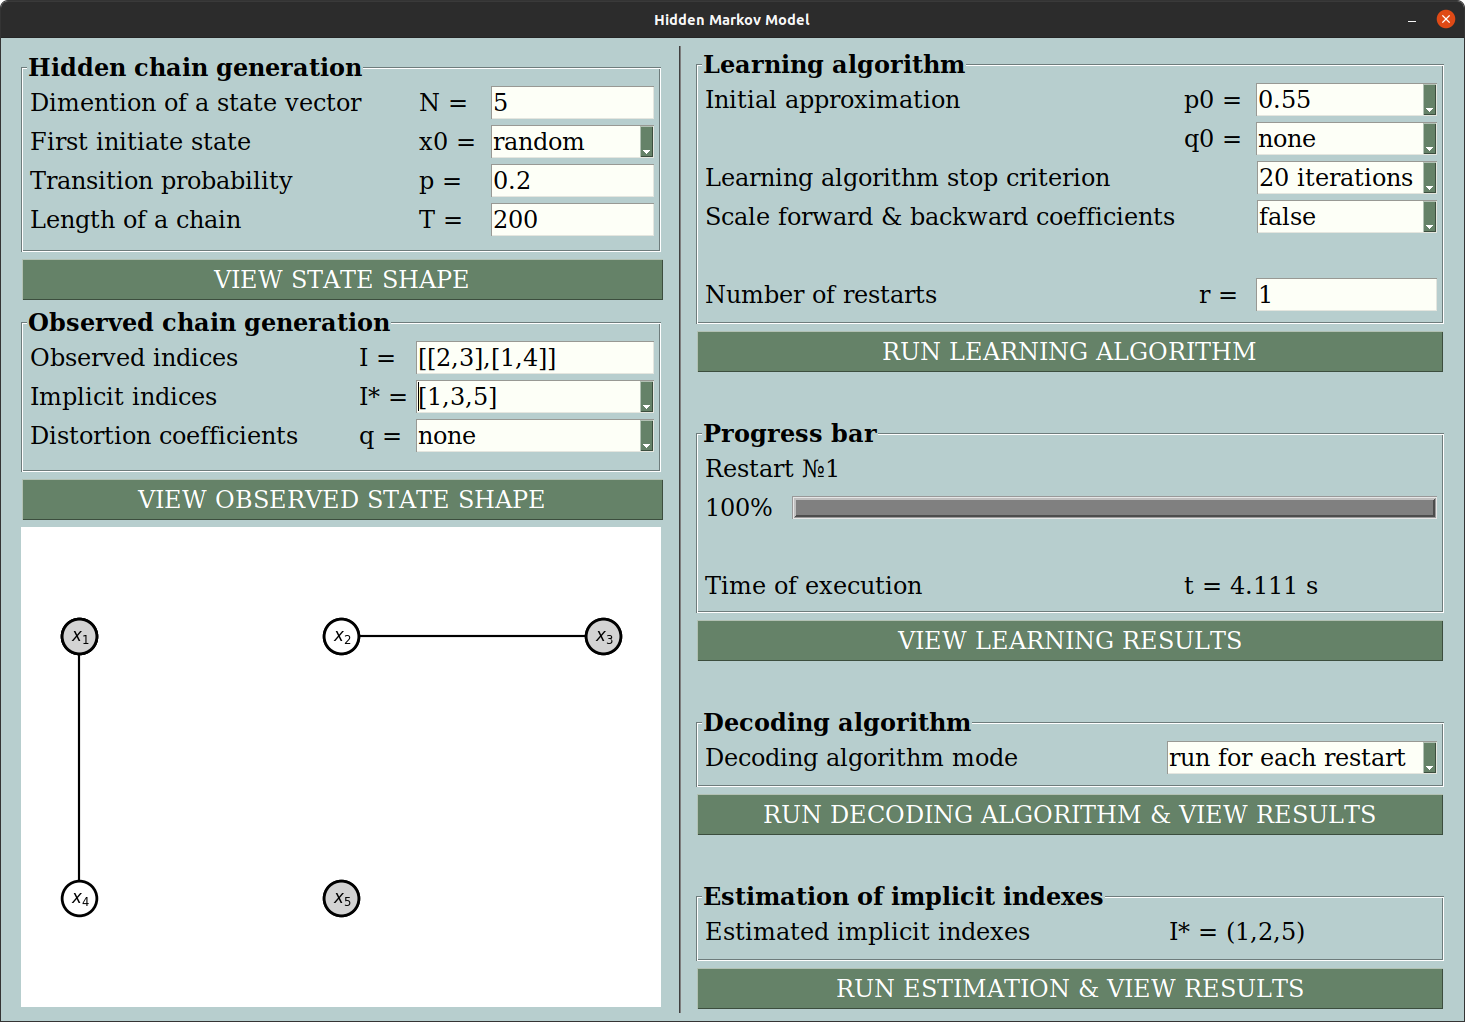
\includegraphics[width=1\linewidth]{Images/GUI.png}
    \caption{Графічний інтерфейс користувача}
    \label{pic: GUI}
\end{figure}

Кожна з відповідних кнопок викликає блоки коду, необхідні для виконання тієї чи іншої задачі. Візуалізація результатів виконується в окремих спливаючих вікнах інтерфейсу у вигляді графіків, наведених у розділі проведення чисельного експерименту.

У лівій нижній частині інтерфейсу схематично зображена конфігурація стану ланцюга: відповідні множини спостережуваних індексів (кожна спостережувана область виокремлюється візуально за з'єднаними ребром вершинами), а також множина неявних індексів, елементи якої позначені сірим кольором.